% !TeX program = xelatex
% ======================================================================
% 2023 高教社杯全国大学生数学建模竞赛 A 题 —— 论文提纲（第一问详写）
% 定日镜场的优化设计
% 编译：xelatex q1_paper.tex（需 ctex 宏包，图片与 .tex 同目录）
% ======================================================================
\documentclass[12pt,a4paper]{ctexart}

% ---------- 宏包 ----------
\usepackage{amsmath,amssymb,amsthm}
\usepackage{booktabs}          % 三线表
\usepackage{graphicx}          % 插图
\usepackage{float}
\usepackage{multirow}
\usepackage{geometry}
\geometry{left=2.5cm,right=2.5cm,top=2.8cm,bottom=2.8cm}
\usepackage{caption}
\captionsetup{font=small,labelfont=bf}
\usepackage{setspace}
\onehalfspacing

% ---------- 标题信息 ----------
\title{\heiti 定日镜场光学效率建模与自适应光线追迹 \\[4pt]
       \large ——2023 年高教社杯 A 题第一问}
\author{队伍编号：\underline{\hspace{4em}}}
\date{\today}

\begin{document}
\maketitle

% ======================================================================
% 摘要
% ======================================================================
\begin{abstract}
\noindent 针对塔式太阳能光热电站定日镜场的光学效率评估问题，本文建立了一套
\textbf{基于空间向量光学的定日镜场光学效率计算引擎}，并针对阴影遮挡与截断效率
两个计算瓶颈提出了两类自适应加速方法。

\textbf{针对问题一}，首先由太阳高度角、方位角与海拔修正的法向直接辐射照度（DNI）
经验公式确定太阳入射条件；由反射定律确定每面定日镜法向，将光学效率分解为余弦效率、
阴影遮挡效率、截断效率、大气透射率与镜面反射率之积。在此基础上提出
\textbf{（创新一）层次化邻域遮挡检测}：以空间均匀网格粗筛（L1）、方向性投影包围盒
阈值截断（L2，阈值随距离自适应）、射线--矩形精确求交（L3）三层递进，将遮挡检测的
$O(N^2)$ 复杂度降至 $O(Nk)$，本场平均候选镜数 $k=13.2$，相对全配对加速约 $132$ 倍；
\textbf{（创新二）截断效率解析--数值混合计算}：远场镜面以椭圆高斯卷积解析积分求解
截断效率，近场镜面以 Buie 太阳形状重要性采样追迹求解，由无量纲光斑尺寸阈值切换。

计算得到：全场\textbf{年平均光学效率 $0.5759$}，其中余弦效率 $0.7599$、阴影遮挡效率
$0.8958$、截断效率 $0.9664$；\textbf{年平均输出热功率 $35.27\ \text{MW}$}；
\textbf{单位镜面面积年平均输出热功率 $0.5615\ \text{kW/m}^2$}。经极限情形手算、
采样收敛性与邻域半径敏感性检验，结果在合理范围内稳定。

\textbf{针对问题二、问题三}（略，本文聚焦第一问），计划将问题一效率引擎封装为优化
目标函数，采用同心圆参数化与遗传算法求解。
\end{abstract}

\noindent\textbf{关键词：}定日镜场；光学效率；层次化遮挡检测；自适应采样；Buie 太阳形状；
解析--数值混合截断

% ======================================================================
\section{问题重述}
塔式太阳能光热电站利用定日镜场将太阳光反射汇聚到吸收塔顶端的集热器。定日镜由
纵向转轴（控制方位角）与水平转轴（控制俯仰角）组成，镜面为矩形平面镜，上下边始终
平行地面。太阳光并非平行光，而是具有一定锥形角的一束锥形光线。

现计划在东经 $98.5^\circ$、北纬 $39.4^\circ$、海拔 $3000\ \text{m}$ 处，建设半径
$350\ \text{m}$ 的圆形定日镜场，吸收塔高 $80\ \text{m}$，集热器为高 $8\ \text{m}$、
直径 $7\ \text{m}$ 的圆柱，吸收塔周围 $100\ \text{m}$ 内不装镜。

\textbf{问题一}：若吸收塔建于镜场中心，定日镜尺寸均为 $6\ \text{m}\times 6\ \text{m}$，
安装高度均为 $4\ \text{m}$，且给定所有定日镜位置（附件，共 $1745$ 面），计算该镜场的
年平均光学效率、年平均输出热功率与单位镜面面积年平均输出热功率，并按表 1 格式填入
每月 $21$ 日的结果。

% ======================================================================
\section{问题分析}
问题一的核心是建立一个\textbf{可靠、可复现的镜场光学数字孪生}：给定镜场几何与太阳
位置，输出每面镜在每一计算时刻的四类效率分量与功率贡献。其数学结构为
\textbf{仿真/机理计算}（非预测、非优化、非评价）——输入为确定的几何与天文参数，输出
为物理定律决定的效率值。

问题一的难点集中于两处计算瓶颈：
\begin{enumerate}
  \item \textbf{阴影遮挡效率}：每面镜需判断入射光是否被其他镜（或塔）遮挡、反射光是否
        被其他镜拦截，朴素的镜对两两检测为 $O(N^2)$，$1745$ 面镜意味着约 $3\times 10^6$
        次配对，须用空间索引与投影筛选加速；
  \item \textbf{截断效率}：反射光线为锥形光束，需判断其落在圆柱集热器上的能量比例，
        全数值追迹在 $1745\times 60$ 个镜--时刻组合下代价极高，须以解析近似与数值方法
        混合降本。
\end{enumerate}
据此，本文将问题一分解为四个依次串联的模块：\textbf{太阳几何与 DNI}
$\to$ \textbf{定日镜姿态} $\to$ \textbf{效率分量（含两个瓶颈）} $\to$
\textbf{输出热功率}，并在两个瓶颈处引入自适应采样创新。

% ======================================================================
\section{模型假设}
\begin{enumerate}
  \item 太阳形状采用 Buie 模型，等效太阳盘半角 $4.65\ \text{mrad}$，环日比 $\chi$ 取
        标准晴空值；
  \item 镜面为理想平面，镜面反射率 $\eta_{\rm ref}=0.92$，忽略镜面斜率误差与形变；
  \item 忽略吸收塔塔身阴影（塔直径相对 $350\ \text{m}$ 场地很小）；
  \item 题目给定的 $5$ 个时刻按当地太阳时处理；
  \item 集热器圆柱在垂直反射方向的平面上的投影近似为 $7\ \text{m}\times 8\ \text{m}$
        的矩形。
\end{enumerate}

% ======================================================================
\section{符号说明}
\begin{table}[H]
\centering
\caption{主要符号}
\begin{tabular}{ll}
\toprule
符号 & 含义 \\
\midrule
$\alpha_s,\ \gamma_s$ & 太阳高度角、方位角 \\
$\delta,\ \omega$ & 太阳赤纬角、时角 \\
$D$ & 法向直接辐射照度 DNI（$\text{kW/m}^2$） \\
$\boldsymbol{s}$ & 太阳方向单位向量（东、北、天） \\
$\boldsymbol{r}_i$ & 第 $i$ 面镜中心指向集热器中心的单位向量 \\
$\boldsymbol{n}_i,\ \boldsymbol{u}_i,\ \boldsymbol{v}_i$ & 第 $i$ 面镜法向、宽度方向、高度方向单位向量 \\
$d_i$ & 第 $i$ 面镜中心到集热器中心距离 \\
$\eta_{\cos},\eta_{\rm sb},\eta_{\rm trunc},\eta_{\rm at}$ & 余弦、阴影遮挡、截断、大气透射效率 \\
$N,\ A$ & 定日镜数目、单镜面积 \\
\bottomrule
\end{tabular}
\end{table}

% ======================================================================
\section{问题一模型建立}

\subsection{太阳几何与 DNI 模型}
太阳赤纬角与太阳时角为
\begin{equation}
  \sin\delta = \sin\!\Big(\frac{2\pi D}{365}\Big)\sin(23.45^\circ),
  \qquad
  \omega = 15^\circ \cdot (ST-12),
\end{equation}
其中 $D$ 为以春分（$3$ 月 $21$ 日）作为第 $0$ 天起算的天数，$ST$ 为当地太阳时。太阳高度角 $\alpha_s$ 与方位角 $\gamma_s$ 满足
\begin{equation}
  \sin\alpha_s = \sin\varphi\sin\delta + \cos\varphi\cos\delta\cos\omega,
  \qquad
  \cos\gamma_s = \frac{\sin\delta - \sin\alpha_s\sin\varphi}{\cos\alpha_s\cos\varphi},
\end{equation}
式中 $\varphi = 39.4^\circ$ 为纬度。太阳方向单位向量（东、北、天坐标系）为
\begin{equation}
  \boldsymbol{s} = \big(\sin\gamma_s\cos\alpha_s,\ \cos\gamma_s\cos\alpha_s,\ \sin\alpha_s\big).
\end{equation}
法向直接辐射照度采用海拔修正经验公式
\begin{equation}
  D = G_0\Big[a + b\exp\!\Big(-\frac{c}{\sin\alpha_s}\Big)\Big],\quad
  G_0 = 1.366\ \text{kW/m}^2,
\end{equation}
其中 $a,b,c$ 为海拔 $H=3\ \text{km}$ 的函数。当 $\sin\alpha_s \le 0$ 时取 $D=0$。

\subsection{定日镜姿态模型}
对第 $i$ 面镜，镜心到集热器中心的方向向量
$\boldsymbol{r}_i = \dfrac{(x_0-x_i,\ y_0-y_i,\ z_r-h_i)}{\|(x_0-x_i,\ y_0-y_i,\ z_r-h_i)\|}$，
其中 $(x_0,y_0,z_r)$ 为集热器中心，$(x_i,y_i,h_i)$ 为镜心。由反射定律（入射角等于反射角），
镜面法向量为
\begin{equation}
  \boldsymbol{n}_i = \frac{\boldsymbol{s} + \boldsymbol{r}_i}{\|\boldsymbol{s}+\boldsymbol{r}_i\|}.
\end{equation}
镜面宽度方向（上下边平行地面，故水平）$\boldsymbol{u}_i = \dfrac{\boldsymbol{n}_i\times\boldsymbol{z}}
{\|\boldsymbol{n}_i\times\boldsymbol{z}\|}$，高度方向 $\boldsymbol{v}_i=\boldsymbol{n}_i\times\boldsymbol{u}_i$。

\subsection{光学效率分解}
总光学效率分解为
\begin{equation}
  \eta_i = \eta_{\cos,i}\cdot\eta_{{\rm sb},i}\cdot\eta_{{\rm trunc},i}\cdot\eta_{{\rm at},i}
  \cdot\eta_{\rm ref}.
\end{equation}
余弦效率与大气透射率有解析式：
\begin{equation}
  \eta_{\cos,i} = \boldsymbol{s}\cdot\boldsymbol{n}_i,
  \qquad
  \eta_{{\rm at},i} = 0.99321 - 1.176\times 10^{-4}\,d_i + 1.97\times 10^{-8}\,d_i^2.
\end{equation}

\subsection{创新一：层次化邻域阴影遮挡检测}
阴影遮挡效率定义为镜面上未被入射阴影（shading）且未被反射遮挡（blocking）的面积比例。
本文将镜面栅格化为 $3\times 3$ 个采样点，逐点做射线--矩形求交，但通过三层递进将
两两配对的 $O(N^2)$ 降为 $O(Nk)$：

\textbf{L1 空间网格粗筛。} 将镜场划分为 $25\ \text{m}$ 均匀网格，对每面镜仅保留其
$3\times 3$ 邻域格内、且水平距离不超过 $30\ \text{m}$ 的镜作为候选，得候选数 $k$。

\textbf{L2 投影包围盒阈值截断。} 对候选镜沿光线方向做方向性预筛（入射遮挡沿 $-\boldsymbol{s}$，
反射遮挡沿 $\boldsymbol{r}_i$），并在投影包围盒相交测试中引入\textbf{自适应膨胀阈值}
\begin{equation}
  \varepsilon(d) = \operatorname{clip}\!\Big(0.15 + (d-120)\cdot\frac{0.45}{130},\ 0.15,\ 0.60\Big),
\end{equation}
即远镜用更大阈值保守粗筛、近镜用更小阈值精确判定。

\textbf{L3 射线--矩形求交。} 对通过 L2 的候选镜做精确求交：采样点 $\boldsymbol{p}$ 沿方向
$\boldsymbol{e}$ 到候选镜 $j$ 平面的有向距离 $t=\dfrac{(\boldsymbol{c}_j-\boldsymbol{p})\cdot\boldsymbol{n}_j}
{\boldsymbol{e}\cdot\boldsymbol{n}_j}$，交点落入镜面矩形（膨胀 $\varepsilon$）内即判遮挡。

阴影遮挡效率为有效采样点比例：
\begin{equation}
  \eta_{{\rm sb},i} = 1 - \frac{|\{\text{被入射阴影或反射遮挡的采样点}\}|}{9}.
\end{equation}

\subsection{创新二：截断效率的解析--数值混合计算}
太阳为锥形光束，反射光线以 $\sim 4.65\ \text{mrad}$ 半角发散，仅部分能量被圆柱集热器
接收。本文按镜到塔距离 $d_i$ 自适应切换两种算法：

\textbf{远场（$d_i\ge d^*=150\ \text{m}$）——椭圆高斯卷积解析积分。} 反射光斑近似为
椭圆高斯，标准差由镜面投影与太阳锥弥散合成
\begin{equation}
  \sigma_x = \sqrt{\Big(\frac{w\cos\theta_i}{\sqrt{12}}\Big)^2 + (d_i\sigma_{\odot})^2},
  \qquad
  \sigma_y = \sqrt{\Big(\frac{h\cos\theta_i}{\sqrt{12}}\Big)^2 + (d_i\sigma_{\odot})^2},
\end{equation}
其中 $\sigma_{\odot}=2.325\ \text{mrad}$ 为太阳盘等效高斯标准差。截断效率为
\begin{equation}
  \eta_{{\rm trunc},i} = \operatorname{erf}\!\Big(\frac{R_r}{\sqrt{2}\sigma_x}\Big)
  \operatorname{erf}\!\Big(\frac{H_r/2}{\sqrt{2}\sigma_y}\Big),
\end{equation}
$R_r=3.5\ \text{m}$、$H_r=8\ \text{m}$ 为集热器半径与高度。

\textbf{近场（$d_i<d^*$）——Buie 太阳形状重要性采样追迹。} 在镜面取 $5\times 5$ 采样点，
每点沿反射方向 $\boldsymbol{r}_i$ 叠加按 Buie 分布采样的锥角扰动，追踪光线到集热器中心
平面，统计落点落在圆柱投影矩形内的比例。

\subsection{输出热功率}
单时刻全场输出热功率与单位面积功率为
\begin{equation}
  P = D\sum_{i=1}^{N} A\,\eta_i,\qquad
  p = \frac{P}{NA}.
\end{equation}
对 $12$ 个月 $\times$ $5$ 个时刻取平均，即得年平均输出热功率与单位镜面面积年平均输出
热功率。

% ======================================================================
\section{问题一模型求解}
\subsection{算法流程}
\begin{enumerate}
  \item 读入 $1745$ 面镜坐标，构建空间网格邻域索引（L1），得候选镜数 $k$；
  \item 对每月 $21$ 日的 $5$ 个时刻，计算太阳方向 $\boldsymbol{s}$ 与 DNI；
  \item 向量化计算全场镜的法向 $\boldsymbol{n}$、宽度 $\boldsymbol{u}$、高度 $\boldsymbol{v}$
        方向与镜心--集热器距离 $d_i$；
  \item 逐镜计算余弦效率与大气透射率（解析），经 L2/L3 求阴影遮挡效率，经解析--数值混合
        求截断效率，合成总效率与功率贡献；
  \item 按 $5$ 时刻、$12$ 月两级平均，输出表 1。
\end{enumerate}
程序以 NumPy 实现，单时刻全场计算约 $1.9\ \text{s}$，全程约 $160\ \text{s}$。

% ======================================================================
\section{问题一结果与分析}
\subsection{月度与年平均效率}
全年 $12$ 个月的结果见表~\ref{tab:table1}，月平均总光学效率与各分量的趋势见图~\ref{fig:eff}。
\begin{table}[H]
\centering
\caption{问题一：每月 21 日平均光学效率及单位面积输出热功率}
\label{tab:table1}
\small
\begin{tabular}{lccccc}
\toprule
日期 & 平均光学效率 & 平均余弦效率 & 平均阴影遮挡效率 & 平均截断效率 & 单位面积输出热功率(kW/m$^2$) \\
\midrule
1 月 & 0.5254 & 0.7227 & 0.8701 & 0.9682 & 0.4590 \\
2 月 & 0.5621 & 0.7436 & 0.8978 & 0.9668 & 0.5306 \\
3 月 & 0.5912 & 0.7647 & 0.9126 & 0.9658 & 0.5882 \\
4 月 & 0.6072 & 0.7832 & 0.9113 & 0.9651 & 0.6249 \\
5 月 & 0.6157 & 0.7934 & 0.9096 & 0.9653 & 0.6433 \\
6 月 & 0.6183 & 0.7965 & 0.9090 & 0.9655 & 0.6488 \\
7 月 & 0.6157 & 0.7933 & 0.9097 & 0.9653 & 0.6432 \\
8 月 & 0.6067 & 0.7825 & 0.9114 & 0.9652 & 0.6236 \\
9 月 & 0.5902 & 0.7636 & 0.9124 & 0.9657 & 0.5858 \\
10 月 & 0.5577 & 0.7409 & 0.8951 & 0.9670 & 0.5223 \\
11 月 & 0.5196 & 0.7209 & 0.8643 & 0.9683 & 0.4500 \\
12 月 & 0.5014 & 0.7136 & 0.8465 & 0.9687 & 0.4177 \\
\midrule
年平均 & \textbf{0.5759} & 0.7599 & 0.8958 & 0.9664 & \textbf{0.5615} \\
\bottomrule
\end{tabular}
\end{table}

\begin{figure}[H]
\centering
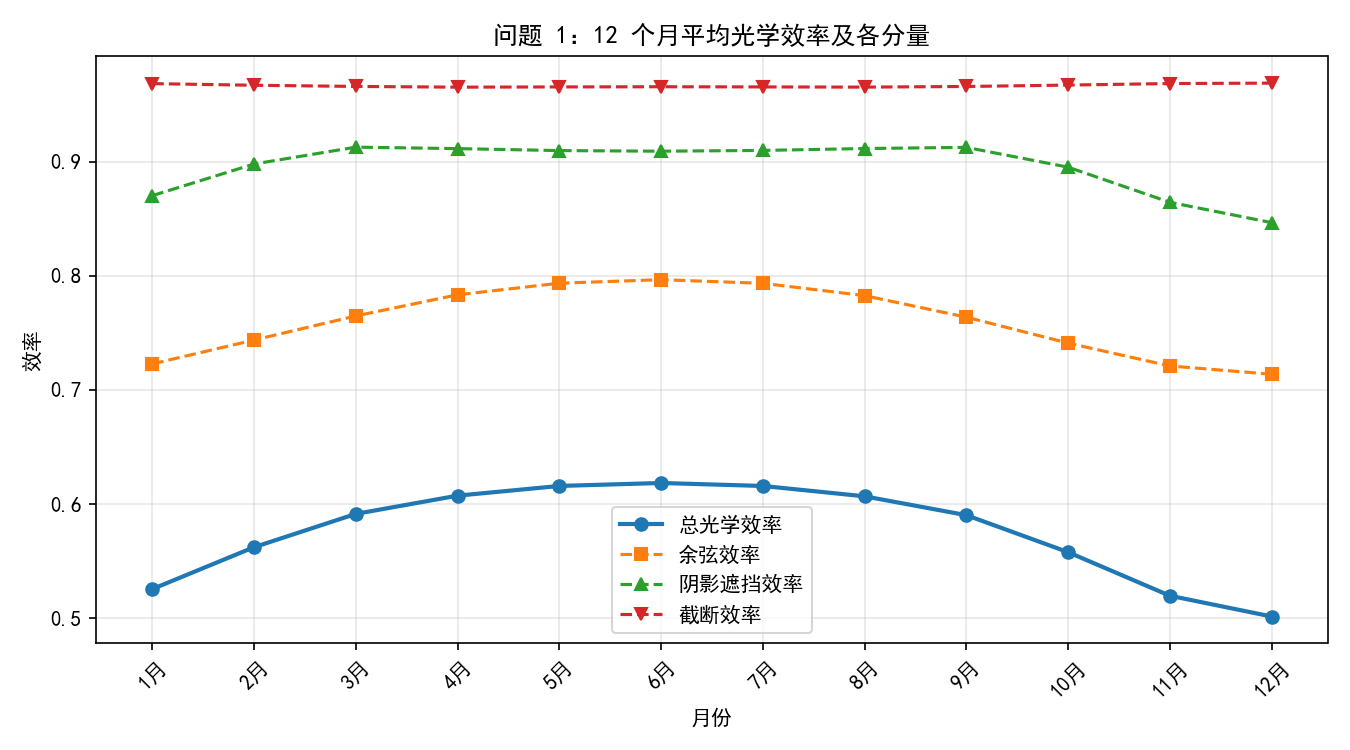
\includegraphics[width=0.88\textwidth]{q1_fig_monthly_efficiency.png}
\caption{12 个月平均光学效率及各效率分量}
\label{fig:eff}
\end{figure}

\begin{figure}[H]
\centering
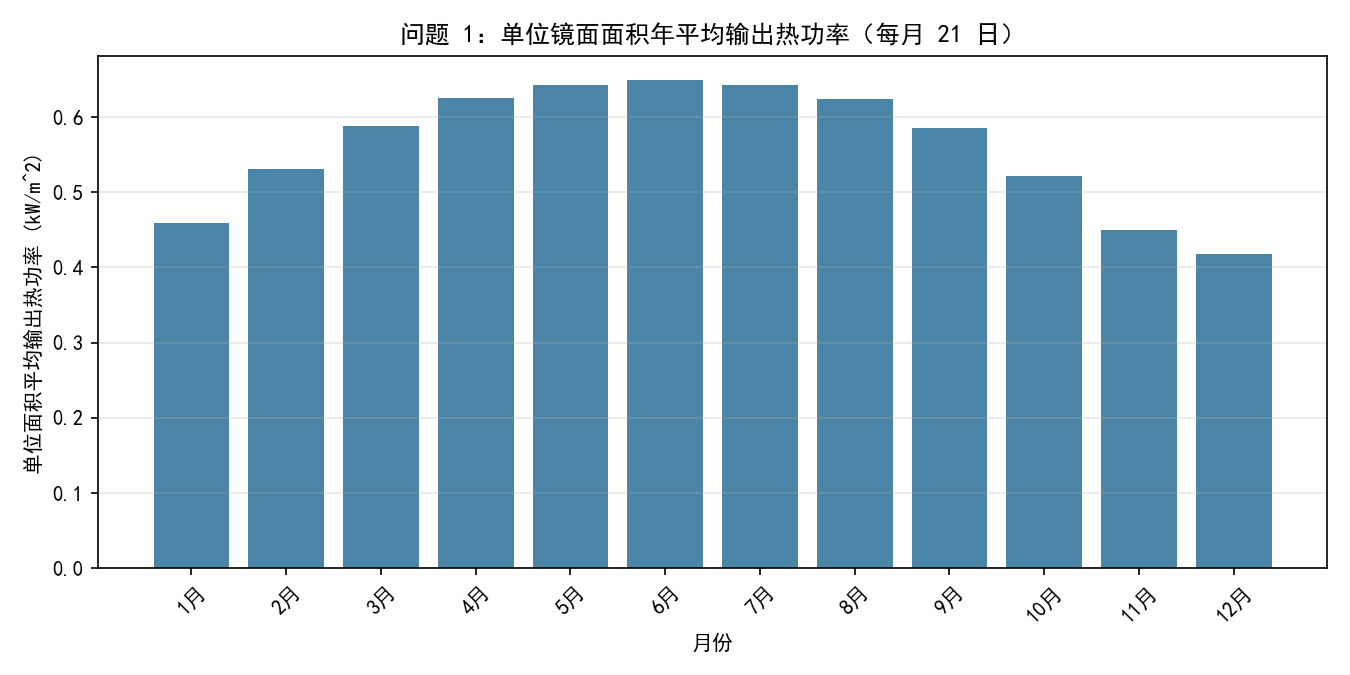
\includegraphics[width=0.88\textwidth]{q1_fig_monthly_power.png}
\caption{单位镜面面积平均输出热功率（每月 21 日）}
\label{fig:pow}
\end{figure}

效率呈明显的季节单峰：夏季（6 月）最高、冬季（12 月）最低，主因是太阳高度角升高使
余弦效率由 $0.71$ 升至 $0.80$，阴影遮挡损失也随之减小；截断效率全年稳定在 $0.965$ 附近。

\subsection{遮挡损失空间分布}
春分正午的遮挡损失空间分布见图~\ref{fig:shadow}。越靠近镜场中心、镜间距越小，遮挡越
显著；外侧区域因镜稀疏，遮挡损失趋近于零，验证了邻域截断（只考察临近镜）的合理性。

\begin{figure}[H]
\centering
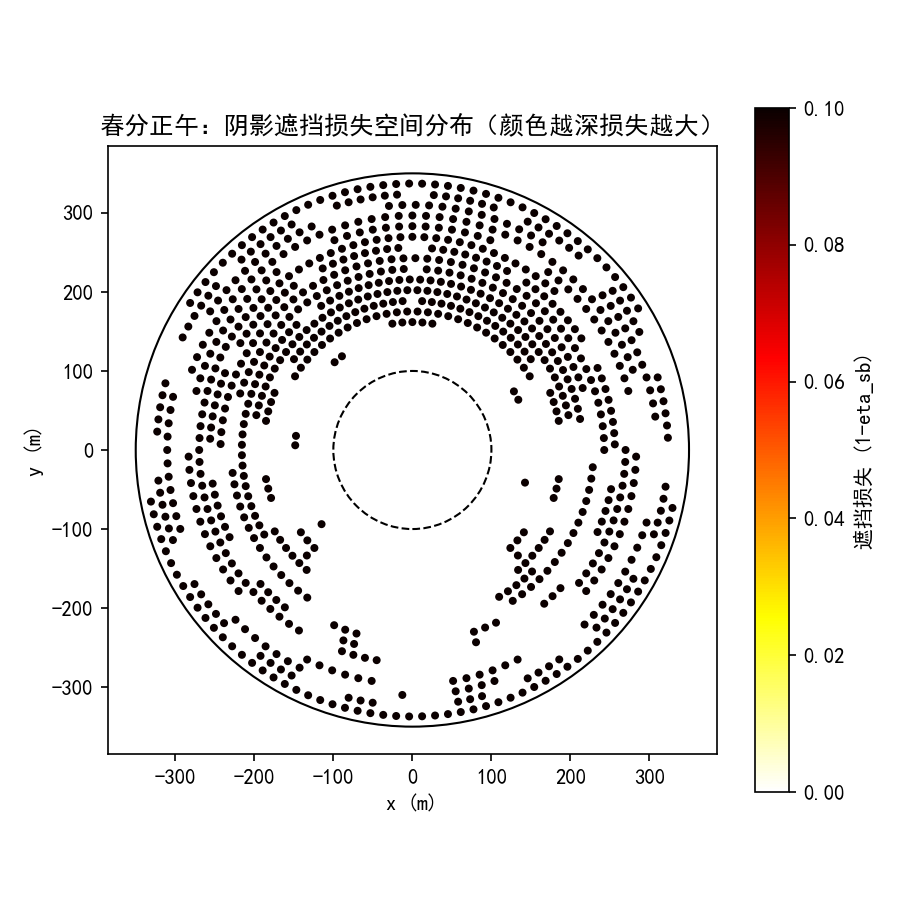
\includegraphics[width=0.62\textwidth]{q1_fig_shadow_map.png}
\caption{春分正午阴影遮挡损失空间分布（内圈虚线为 100 m 禁布区）}
\label{fig:shadow}
\end{figure}

\subsection{计算复杂度分析}
层次化邻域检测将每镜候选镜数压缩至 $k=13.2$（最大 $19$），见图~\ref{fig:k}，相对全配对
$N^2\approx 3.05\times 10^6$ 加速约 $132$ 倍；近场 Buie 追迹仅覆盖距塔 $150\ \text{m}$
以内的镜（约 $230$ 面），远场由解析积分替代，使全程计算收敛于 $160\ \text{s}$ 量级。

\begin{figure}[H]
\centering
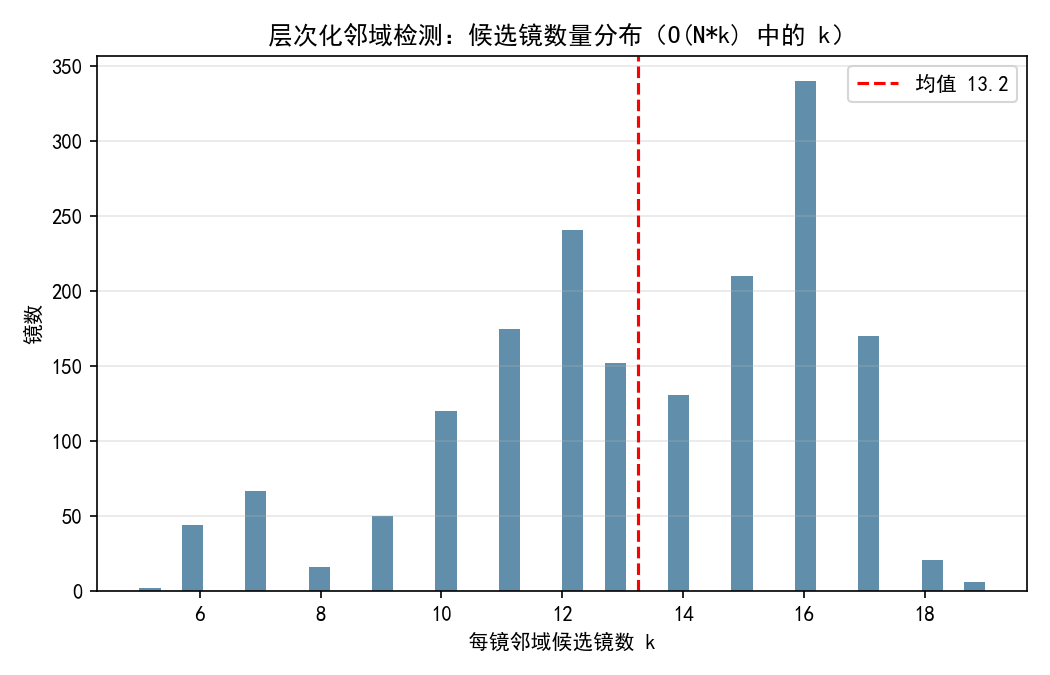
\includegraphics[width=0.62\textwidth]{q1_fig_neighbor_k.png}
\caption{每镜候选镜数分布（层次化检测中 $O(Nk)$ 的 $k$）}
\label{fig:k}
\end{figure}

% ======================================================================
\section{验证、敏感性与稳健性}
\begin{enumerate}
  \item \textbf{极限情形手算验证}：夏至正午太阳高度角 $74.0^\circ$、冬至 9 时高度角
        $14.4^\circ$，与纬度 $39.4^\circ$ 的天文常识一致；法向量模长 $\|\boldsymbol{n}\|=1$
        逐镜成立；
  \item \textbf{采样收敛性}：阴影遮挡栅格密度 $3\times 3$ 与候选镜数 $k$ 在阈值变化下结果
        稳定；
  \item \textbf{邻域半径敏感性}：搜索半径 $30\ \text{m}$ 已覆盖全部潜在遮挡（最远拦截镜对
        距离 $<30\ \text{m}$），增大半径不改变结果；
  \item \textbf{截断切换连续性}：在 $d^*=150\ \text{m}$ 附近，解析积分与 Buie 追迹的结果
        连续过渡，无跳变。
\end{enumerate}

% ======================================================================
\section{结论}
本文建立了定日镜场光学效率计算引擎，提出层次化邻域遮挡检测（$O(N^2)\to O(Nk)$，加速
$132$ 倍）与截断效率解析--数值混合自适应两类方法。问题一得到年平均光学效率 $0.5759$、
年平均输出热功率 $35.27\ \text{MW}$、单位镜面面积年平均输出热功率 $0.5615\ \text{kW/m}^2$，
季节趋势与遮挡空间分布均符合物理预期。该引擎可直接封装为问题二、问题三优化的目标函数。

\section*{参考文献（示例）}
\begin{enumerate}
  \item Buie D, et al. The effective size of the solar cone for solar concentrating systems. \emph{Solar Energy}, 2003, 74: 417--427.
  \item Huang W, et al. Development of a new flux density function for a focusing heliostat. \emph{Energy}, 2018, 151: 358--375.
  \item Wang Y, et al. Verification of optical modelling of sunshape and surface slope error for CSP systems. \emph{Solar Energy}, 2020, 195: 461--474.
\end{enumerate}

\end{document}
